% ca. 20%

\section{Einleitung} 

In der heutigen Softwareentwicklung gewinnen strukturierte Schnittstellen zwischen Systemkomponenten zunehmend an Bedeutung. 
Insbesondere Web-APIs bilden die Essenz vieler verteilter Anwendungen, bei denen unterschiedliche Systeme, etwa Frontend- und Backend-Komponenten, 
zuverlässig miteinander kommunizieren müssen.
Ein zentrales Element solcher APIs ist die präzise Beschreibung der übermittelten Daten. 
Auch wenn die Typisierung hierbei eine essenzielle Rolle spielt, um Fehler zu vermeiden, 
Entwicklungsprozesse zu standardisieren und die Wartbarkeit langfristig zu sichern,
ist die Definition der Schnittstellen nicht Trivial.
In der folgenden Arbeit soll aufgezeigt werden, wie Schnittstellen strukturiert definiert werden können und welche
Tools existieren um diese Definition konsistent über Systeme hinweg durchzuführen.

Diese Arbeit richtet sich an Leser*innen mit technischem Hintergrund im Bereich der Softwareentwicklung, 
insbesondere an Softwareentwickler*innen und -architekt*innen, die mit der Definition, Analyse oder Nutzung von Web-APIs befasst sind.
Darüber hinaus ist sie auch für Informatikstudent*innen geeignet,
die bereits Grundkenntnisse im Bereich Typensysteme besitzen und diese auf in der Praxis in Bezug auf Schnittstellen anwenden möchten,
um die Wartbarkeit von ihren APIs zu erhöhen.


\subsection{Grundlagen}

Für das Verständnis der Arbeit wird angenommen, dass Leser*innen ein Grundlegendes Wissen über Webanwendungen sowie REST-APIs besitzen.
Auch wenn kein tieferes Wissen diesbezüglich erforderlich ist, hilft es dennoch wenn Begrifflichkeiten und Grundlegende Konzepte wie 
Endpunkte, HTTP-Methoden und Anfrage/Antwortkörper bekannt sind.

Es sollten Grundlegende Kenntnisse über die Struktur von JSON vorlegen, da dies als Beispiel sowie für die OpenAPI Schemata verwendet wird.

Kenntnisse über TypeScript sind hilfreich, aber nicht erforderlich. Die Typentheoretischen Begriffe und Konzepte werden in der Arbeit erläutert.
Hierfür ist ein Basiswissen über die Mengenlehre förderlich.

Es ist nicht nötig, dass Leser*innen bereits über ein Wissen zu OpenAPI oder API Schemata verfügen, da dies das Thema der Arbeit ist.

\subsection{Problemstellung}

In der Praxis besteht häufig eine Diskrepanz zwischen der dokumentierten API und ihrer tatsächlichen Implementierung.
Diese Abweichungen können zu Laufzeitfehlern, Missverständnissen in der Entwicklung und erhöhtem Wartungsaufwand führen, insbesondere dann, wenn keine oder nur unzureichende Typisierung verwendet wird. 
Dynamisch typisierte Systeme sind in dieser Hinsicht besonders anfällig, da Fehler oft erst spät, beispielsweise zur Laufzeit oder beim Testen, erkannt werden.
Dies ist der Grund, warum Sprachen wie TypeScript existieren, welche versuchen existierende Sprachen um Typsysteme anzureichern.

\begin{figure}[H]
  \centering
  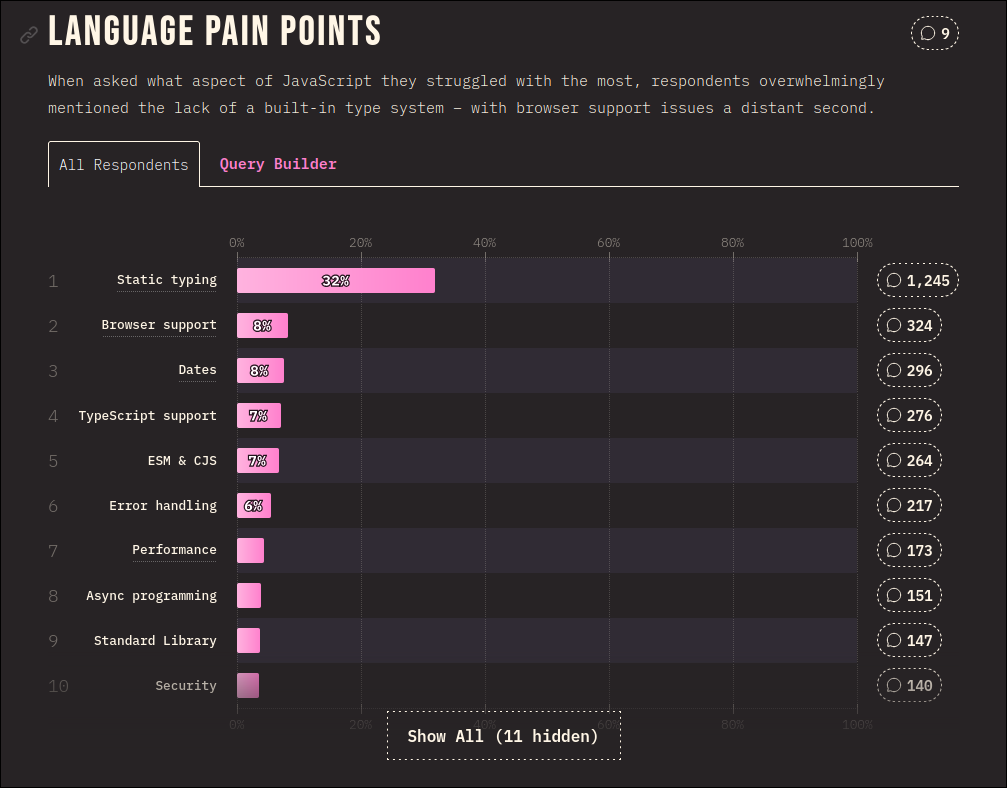
\includegraphics[width=0.9\textwidth]{state_of_js}
  \caption{32\% der Befragten in der \textquote{State of JavaScript 2024} Umfrage gaben an das (fehlende) statische Typisierung einer ihrer größten Probleme mit der Sprache sei \cite{Greif_Burel_2024}}
\end{figure}

Selbst bei Verwendung von statisch typisierten Sprachen bleibt die manuelle Synchronisierung zwischen API-Dokumentation und Code eine fehleranfällige Aufgabe. 
Dies betrifft sowohl Backend-Entwickler*innen, die Schnittstellen bereitstellen, als auch Frontend-Entwickler*innen, 
die auf diese Schnittstellen zugreifen und korrekte Datenannahmen treffen müssen.
Bei Diskrepanzen zwischen den Definitionen kann es zu Problemen führen, bei denen Nutzer der Website unerwartete Fehler erhalten was ein Betriebsrisiko für
das Softwareprodukt bedeutet. Um dies zu vermeiden sind eventuell End-To-End tests nötig, welche kostenaufwendig und schwer zu pflegen sind.

\subsection{Ziel der Arbeit}

Ziel dieser Arbeit ist es, die Relevanz und den Nutzen von Typensystemen bei der Modellierung und Beschreibung moderner Web-APIs aufzuzeigen. 
Im Mittelpunkt steht dabei die Analyse, wie typentheoretische Konzepte, insbesondere Produkt- und Summentypen, auf API-Schnittstellen übertragen 
und durch Standards wie OpenAPI formalisiert werden können.

Dabei wird exemplarisch untersucht, wie sich aus API-Schemata typisierte Datenstrukturen generieren lassen, um sowohl Konsistenz als auch 
Typsicherheit für das Softwareprodukt zu gewährleisten und die Wartbarkeit und Fehlerresistenz zu erhöhen.
Die Arbeit veranschaulicht diese Zusammenhänge anhand konkreter Beispiele und Anwendungsfälle.

Insgesamt soll die Arbeit Architekten von Webanwendungen dabei helfen API-Schnittstellen eindeutig zu definieren und die in der Arbeit erwähnten Tools sinnvoll einzusetzen,
um konsistente, klar definierte und typsichere Endpunkte zu schreiben.
Die Arbeit soll primär als Startpunkt gelten und die Tools nicht im Detail beschreiben oder Anweisungen geben, wie diese zu benutzen sind. Es soll ausschließlich dargestellt
werden, was für ein Lösungsansatz für das gegebene Problem existiert.
